\chapter{利润最大化}
\label{sec:profit-maximization}

\section{最优产量选择}
假定总收益$TR(q)$、总成本$TC(q)$均仅为产量$q$的函数,则总利润$\pi(q)$函数可以表示为
\[
\pi (q) = TR(q) - TC(q)
\]
欲图得到最大利润,则要找到$\pi(q)$的极大值,其一阶条件必须满足:
\[
\frac{{d\pi}}{{dq}}= \frac{{dTR}}{{dq}} - \frac{{dTC}}{{dq}}= MR - MC = 0
\]
并且满足一阶条件的产量$q^*$必须满足二阶条件:
\[
{\left. {\frac{{{d^2}\pi }}{{d{q^2}}}} \right|_{q = q^*}} = {\left. {\frac{{d\pi '}}{{dq}}} \right|_{q = q^*}} < 0
\]

\begin{figure}[!h]
\begin{shaded*}
  \begin{minipage}[t]{0.5\linewidth} 
    \centering 
	    \vspace{0pt}
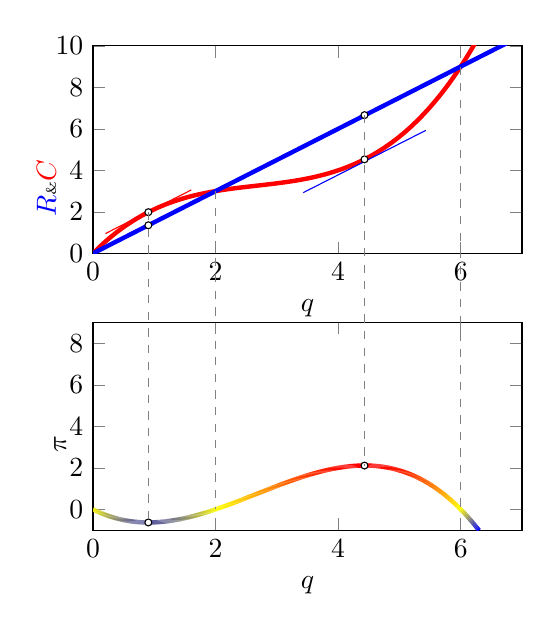
\begin{tikzpicture}
\begin{axis}[
	xmin=0,xmax=7,ymin=0,ymax=10,
	height=120pt,width=200pt,
	xlabel style={below},xlabel=$q$,
	ylabel style={left},ylabel=$\textcolor{blue}{R}${\tiny$\&$}$\textcolor{red}{C}$,
	samples=400]
\addplot[red,ultra thick,domain=0:8] {(x^3)/8-x^2+3*x};
\addplot[blue,ultra thick,domain=0:8] {1.5*x};
\addplot[blue,thin,domain=3.43:5.43] {1.5*x-2.22};
\addplot[red,thin,domain=0.203:1.603] {1.5*x+0.65};
\addplot[only marks,forget plot,black,mark options={mark size=1.25pt,fill=white},mark=*]
	coordinates {
		(4.43,4.53)
		(4.43,6.66)
		(0.903,1.985)
		(0.903,1.354)	};
\coordinate (A) at (axis cs:4.43,6.66);
\coordinate (B) at (axis cs:4.43,4.53);
\coordinate (C) at (axis cs:0.903,1.985);
\coordinate (D) at (axis cs:2,3);
\coordinate (E) at (axis cs:6,9);
\end{axis}
\begin{axis}[
	yshift=-100pt,height=120pt,width=200pt,
	xmin=0,xmax=7,ymin=-1,ymax=9,
	xlabel style={below},xlabel=$q$,
	ylabel style={left},ylabel=$\pi$,
	samples=400]
\addplot[yellow,ultra thick,domain=0:6.3,colormap name=hot,mesh] {-1.5*x+x^2-(x^3)/8};
\addplot[only marks,forget plot,black,mark options={mark size=1.25pt,fill=white},mark=*]
	coordinates {(4.43,2.11) (0.903,-0.631)	};
\coordinate (AN) at (axis cs:4.43,2.11);
\coordinate (CN) at (axis cs:0.903,-0.631);
\coordinate (DN) at (axis cs:2,0);
\coordinate (EN) at (axis cs:6,0);
\end{axis}
\draw[gray,thin,dashed] (A) -- (AN);
\draw[gray,thin,dashed] (C) -- (CN);
\draw[gray,thin,dashed] (D) -- (DN);
\draw[gray,thin,dashed] (E) -- (EN);
\end{tikzpicture}
\end{minipage}% 
\begin{minipage}[t]{0.5\linewidth} 
\vspace{100pt}
\caption{利润最大化的条件}
\label{fig:profit-maxinization-condition}
{\kaishu\small  利润最大化的产量点,收益曲线的切线与成本曲线的切线是平行的,还要排除$C>R$的点。注意:图示中产品价格是固定的,故而收益曲线为直线。}
\end{minipage} 
\end{shaded*}
\end{figure}

\section{库恩—塔克条件}
\label{sec:Kuhn-Tucker-theorem}
\index{Kuhn--Tucker Theorem 库恩—塔克定理}
\index{Kuhn--Tucker condition 库恩—塔克条件}


\begin{figure}[!h]
\colorbox{black!3}{\parbox{\linewidth-2\fboxsep}{%
\centering
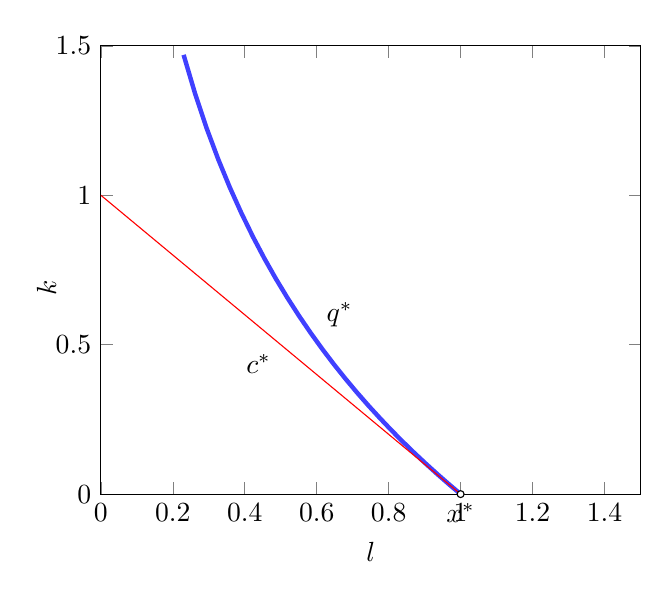
\begin{tikzpicture}
\begin{axis}[
	xmin=0,xmax=1.5,ymin=0,ymax=1.5,
	xlabel style={below},xlabel=$l$,
	ylabel style={left},ylabel=$k$,
	extra x ticks={1},
	extra x tick labels={{$x^*$}}]
\addplot[domain=0.23:1,draw=blue!75,ultra thick] {-ln(x)};
\addplot[red,domain=0:1] {1-x};
\addplot[only marks,forget plot,black,mark options={mark size=1.25pt,fill=white},mark=*] coordinates {(1,0)};
\node[right] at (axis cs:0.6,0.6) {$q^*$};
\node[below left] at (axis cs:0.5,0.5) {$c^*$};
\end{axis}
\end{tikzpicture}

\caption{库恩塔克条件与边角解}
\label{fig:kuhn-tucker-theorem-and-corner-solution}
}}
\end{figure}



\section*{推荐阅读}
\markright{推荐阅读}
\addcontentsline{toc}{section}{\hspace{-2.5em}推荐阅读}


